\chapter{Implementation Protocol} 
\label{sec-protocol} 

This chapter provides details of the implementation of the Kafka protocol, which
acts as basis for all further functionality. The definition of the original
protocol is given as context free grammar for the request and response binary
format \cite{kafka-protocol}. Therefore it seemed likely to adopt the rules of the grammar to our
protocol implementation by map them with the Haskell type system. In a second
step encoding and decoding functionality was implemented for getting messages
from data structure to binary format and backwards. In addition to the protocol,
a client library will be provided to not isolate client implementations from
protocol implementation but also allow to build simple Apache Kafka or HMB
clients in Haskell without touching the protocol at all.

The protocol implementation consists of the following modules: 
\begin{itemize}
    \item {Types: Mapping the protocol definition with Haskell type system. }
    \item {Decode: Provide functions to parse binary data to valid structure. }
    \item {Encode: Provide functions to serialize a given structure to a binary
        format. }
    \item {Client: Provide functions to simplify a Haskell client.}
\end{itemize}

\section{Types}

The design of the Apache Kafka protocol allows to make a distinction between
three kind of types:

\begin{enumerate}
  \item Related to request
  \item Related to response
  \item Related to data (for either request or response but can also be used for
      the \fnurl{Apache Kafka
      Log}{http://kafka.apache.org/documentation.html\#log} component since log
      files (on-disk) hold the same structure) 
\end{enumerate}

As mentioned before, the representation of the protocol structure is implemented
using the Haskell \fnurl{type system}{https://wiki.haskell.org/Type}, more
concrete using data types created for our need using the named fields - also
known as \fnurl{record
syntax}{http://en.wikibooks.org/wiki/Haskell/More_on_datatypes}. Given this, a
further step of abstraction is introduced by creating types for the binary
representation (\ref{subsec:protocol-types-primitive}) of a protocol field, as
described in.

\subsection{Naming convention}

For request and response related types a custom naming convention is introduced
as it is a fact, that not every field of some kind of request or response will
be unique. For more than once, there is a field that will represent a
\textit{topicName} for example. Thus, naming the field \textit{topicName} would
have been the obvious solution but since the record syntax in Haskell won't
allow to use the same name for a field twice - even in different data types -
unique prefixes were defined for each request and response. The following table
provides information about the types related to request or response as well its
prefix:

\begin{table}[H]
\centering
\begin{tabular}{|l|l|l|}
\hline
\textbf{API}            & \textbf{Request (Rq)} & \textbf{Response (Rs)} \\ \hline
Metadata API (Md)       & MetadataRequest       & MetadataResponse       \\ \hline
Produce API (Pr)        & ProduceRequest        & ProduceResponse        \\ \hline
Fetch API (Ft)          & FetchRequest          & FetchResponse          \\ \hline
Offset API (Of)         & OffsetRequest         & OffsetResponse         \\ \hline
Offset Commit API (Ofc) & OffsetCommitRequest   & OffsetCommitResponse   \\ \hline
Offset Fetch API (Oft)  & OffsetFetchRequest    & OffsetFetchResponse    \\ \hline
\end{tabular}
\end{table}

%\subsubsection{Example}
As a result, a typical data type is described as follows, while details are
hidden for demonstration purposes.:

\begin{lstlisting}
-- more
data Partition =
    ----------------------
    -- ProduceRequest (pr)
    ----------------------
    RqPrPartition
    { rqPrPartitionNumber :: !PartitionNumber
    , rqPrMessageSetSize  :: !MessageSetSize
    , rqPrMessageSet      :: [MessageSet]
    }
    |
    ----------------------
    -- FetchRequest (ft)
    ----------------------
    RqFtPartition
    { rqFtPartitionNumber :: !PartitionNumber
    , rqFtFetchOffset     :: !Offset
    , rqFtMaxBytes        :: !MaxBytes
    }
    |
-- more
\end{lstlisting}


\subsection{Batching}
\label{impl-prot-batching}
A significant characteristic of the Kafka protocol is the ability to optimize
efficiency due to the batching of multiple message in one single request. Both
the API to send messages and the API to consume messages always work with a
sequence of messages and not only a single message. It is also possible to batch
messages across multiple topics and partitions. It is task of the client
implementation to use this ability clever but it also can ignore it and sends everything
one at a time. Batching leads to sequences of the same type in one request or response. Within
the protocol format this is defined by an array type. In our protocol
implementation the batching sequences are implemented with Haskell lists which
contains N repetitions of another type. Sequences can also be nested. 

As example, the following grammar rule of the original definition shows the
support of batching in the protocol. A batching sequence of a structure A is
shown as [A]:
\begin{lstlisting}
ProduceRequest => 
    RequiredAcks Timeout [TopicName [Partition MessageSetSize MessageSet]]
\end{lstlisting}

\subsection{Primitive Types}
\label{subsec:protocol-types-primitive}

The actual type for the data fields in the protocol have to match an unsigned
integer type of its length. This can easily be done using the
\fnurl{Data.Word}{http://hackage.haskell.org/package/base-4.7.0.2/docs/Data-Word.html}
library. However, while repetitive writing \textit{WordX} (where is stands for
8-, 16-, 32-, or 64 bit) is rather intuitive, creating aliases using the
\textit{type} keyword will result in better readable code, as well as structure
of the implemented protocol. 

%Sumarized, all protocol related types are size delimited and
%are made up of the following primitive types: 
\begin{table}[H]
    \begin{tabular}{| p{3cm}| p{7cm} | p{5cm} |}
\hline
\textbf{Type} & \textbf{Description} & \textbf{Used Haskell Library} \\ \hline
Fixed Width Primitives     & Signed integers stored in big endian order.
& Data.Word8, Word16, Word32, Word64 \\ \hline
Variable Length Primitives & Consist of a signed integer giving a length N
followed by N bytes of content. A length of -1 indicates null. String uses an
int16 (Data.Word16) for its size, and bytes uses an int32 (Data.Word32).    &
Data.ByteString(.Lazy) \\ \hline
Arrays                     & Repeated structures. Always be encoded as an int32
size containing the length N followed by N,repetitions of the structure which
can itself be made up of other,primitive types & Data.List                          \\ \hline
\end{tabular}
\end{table}

\subsection{Error Codes}
\label{subsec:protocol-types-error-codes}

To handle errors, the protocol specifies error codes they can be sent within a
response message. To adapt those codes, a data type \lstinline{ErrorCode}
deriving from
\fnurl{\lstinline{Enum}}{http://hackage.haskell.org/package/base-4.8.0.0/docs/Prelude.html\#t:Enum} is provided and implicitly represents the
appropriate error code by its order.

\begin{code}
data ErrorCode =
        NoError
      | Unknown
      | OffsetOutOfRange
      | InvalidMessage
      | UnknownTopicOrPartition
      | InvalidMessageSize
      | LeaderNotAvailable
      | NotLeaderForPartition
      | RequestTimedOut
      | BrokerNotAvailable
      | ReplicaNotAvailable
      | MessageSizeTooLarge
      | StaleControllerEpochCode
      | OffsetMetadataTooLargeCode
      | OffsetsLoadInProgressCode
      | ConsumerCoordinatorNotAvailableCode
      | NotCoordinatorForConsumerCodeA
        deriving (Show, Enum)
\end{code}

\subsection{Types related to Request}
A request message is the on-wire format of data which is getting from client to
broker.

Each request message has its same header fields independent for which API they are used. 
The real payload of the request is individual to the particular API which is
used.

\begin{figure}[H]
    \centering
    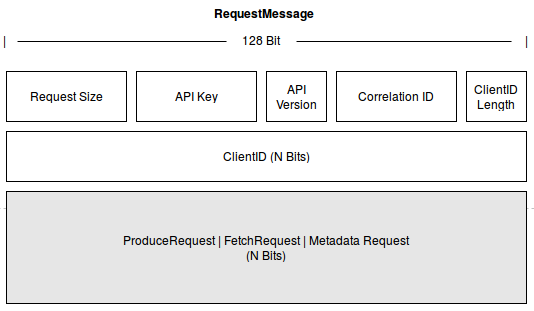
\includegraphics[width=0.7\textwidth]{images/impl-prot-types-requestMessage.png}
    \caption{Format of type RequestMessage}
    \label{fig:impl-prot-types-requestMessage}
\end{figure}

\begin{table}[H]
\centering
\begin{tabular}{ l  l  p{10cm} }
\hline
RequestSize   & Data.Word32     & Gives the size of the subsequent request message in bytes. The client can read requests by first reading this 4 byte size as an integer N and then reading and parsing the subsequent N bytes of the request. \\ \hline
ApiKey        & Data.Word16     & This is a numeric id for the API being invoked                                                                                                                                                              \\ \hline
ApiVersion    & Data.Word16     & Number of element in following list.                                                                                                                                                                          \\ \hline
CorrelationId & Data.Word32     & Will be passed back in the response by the broker unmodified. It is useful for matching request and response between the client and server.                                                                   \\ \hline
StringLength  & Data.Word16     & Length, in bytes, of string ClientId                                                                                                                                                                          \\ \hline
ClientID      & Data.ByteString & Identifier for the client application                                                                                                                                                                         \\ \hline
Request       &                 & API specific Request type (either ProduceRequest, FetchRequest, or others)                                                                                                                                    \\ \hline
\end{tabular}
\end{table}

Regarding to the API key the following numeric codes are already provided by the
protocol implementation (other API's are not implemented yet): 
\begin{table}[h]
    \centering
    \begin{tabular}{ll}
        {\bf API Name}  & {\bf ApiKey Value} \\
        ProduceRequest  & 0                  \\
        FetchRequest    & 1                  \\
        MetadataRequest & 3                 
    \end{tabular}
\end{table}

\subsubsection{ProduceRequest}
\label{subsec:protocol-types-producerequest}

Request Payload for Produce API. Sends MessageSet's (see 
\ref{impl-protocol-types-data}) to the broker. For efficiency it allows sending
message sets intended for many topic partitions in a single request (see
\ref{impl-prot-batching}). MessageSets are not preceded by an int32 like other
array elements in the protocol.

\begin{figure}[H]
    \centering
    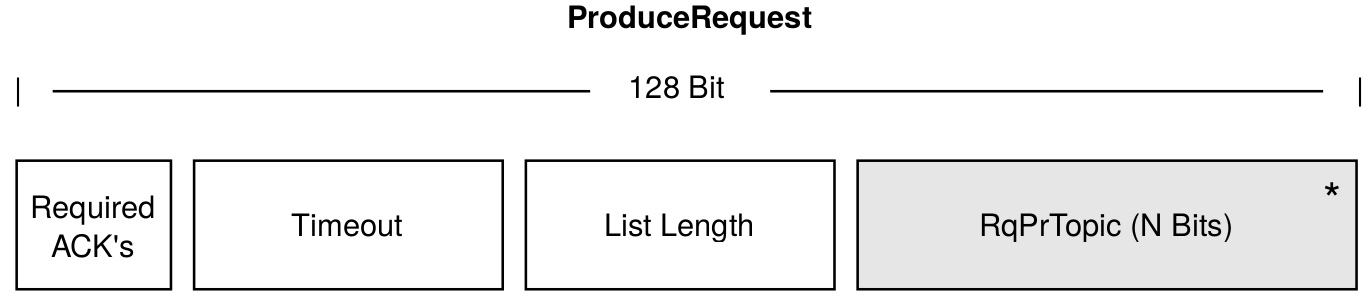
\includegraphics[width=0.7\textwidth]{images/impl-prot-types-produceRequest.png}
    \caption{Format of type ProduceRequest; * = N repetitions }
    \label{fig:impl-prot-types-produceRequest}
\end{figure}

\begin{table}[H]
\centering
\begin{tabular}{ l  l  p{10cm} }
\hline
RequiredAcks  & Data.Word16 & This field indicates how many acknowledgements the broker should receive before responding to the request.                       \\ \hline
Timeout       & Data.Word32 & This provides a maximum time in milliseconds the broker can await the receipt of the number of acknowledgements in RequiredAcks. \\ \hline
ListLength    & Data.Word32 & Number of element in following list.                                                                                             \\ \hline
{[}RqPrTopic{]} & Data.List   & Sequence of RqPrTopics, see below.                                                                                                  \\ \hline
\end{tabular}
\end{table}

A ProduceRequest includes N repetitions of the RqPrTopic type whereas the producer
client is able to send messages for multiple different topics:

\begin{figure}[H]
    \centering
    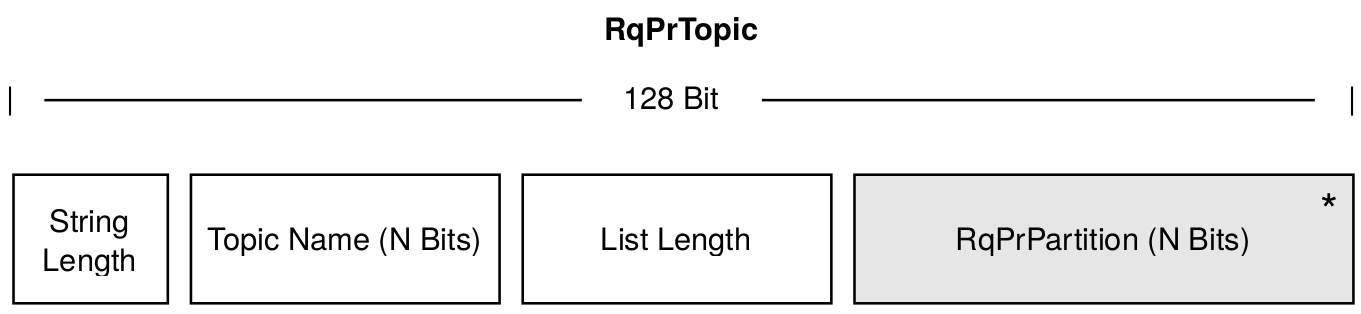
\includegraphics[width=0.7\textwidth]{images/impl-prot-types-prTopic.png}
    \caption{Format of type RqPrTopic; * = N repetitions }
    \label{fig:impl-prot-types-produceRequest}
\end{figure}

\begin{table}[H]
\centering
\begin{tabular}{ l  l  p{10cm} }
\hline
StringLength      & Data.Word16     & Length, in bytes, of string TopicName.              \\ \hline
TopicName         & Data.ByteString & Name of the topic that data is being published to. \\ \hline
ListLength        & Data.Word32     & Number of element in following list.                \\ \hline
[RqPrPartition] & Data.List          & Sequence of PrPartitions, see below.                \\ \hline
\end{tabular}
\end{table}

The RqPrTopic in turn includes N repetitions of the RqPrPartition type
whereas the producer client is able to send message for multiple partitions
within a topic.  

\begin{figure}[H]
    \centering
    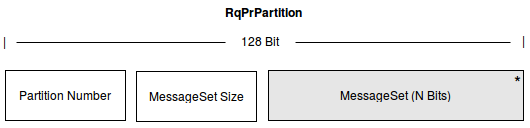
\includegraphics[width=0.7\textwidth]{images/impl-prot-types-prPartition.png}
    \caption{Format of type RqPrTopic; * = N repetitions }
    \label{fig:impl-prot-types-produceRequest}
\end{figure}

\begin{table}[H]
\centering
\begin{tabular}{ l  l  p{11cm} }
\hline
PartitionNumber & Data.Word32 & The partition Id that data is being published to.                                                                                                                                        \\ \hline
MessageSetSize  & Data.Word32 & Sequences of MessageSet's are not preceded by an int32 like other array elements in the protocol. Instead, this field determines the total size, in bytes, of the following MessageSet's. \\ \hline
[MessageSet]      & Data.List      & Finally the RqPrPartition type also holds the actual messages (as defined in \ref{impl-protocol-types-data}.                                                                                \\ \hline
\end{tabular}
\end{table}

\subsubsection{FetchRequest}
\label{subsubsec:protocol-fetchrequest}

Request Payload for Fetch API. Fetchs chunk of one or more logs for some
topic-partitions. Defines a starting offset at which to begin fetch. 

\begin{figure}[H]
    \centering
    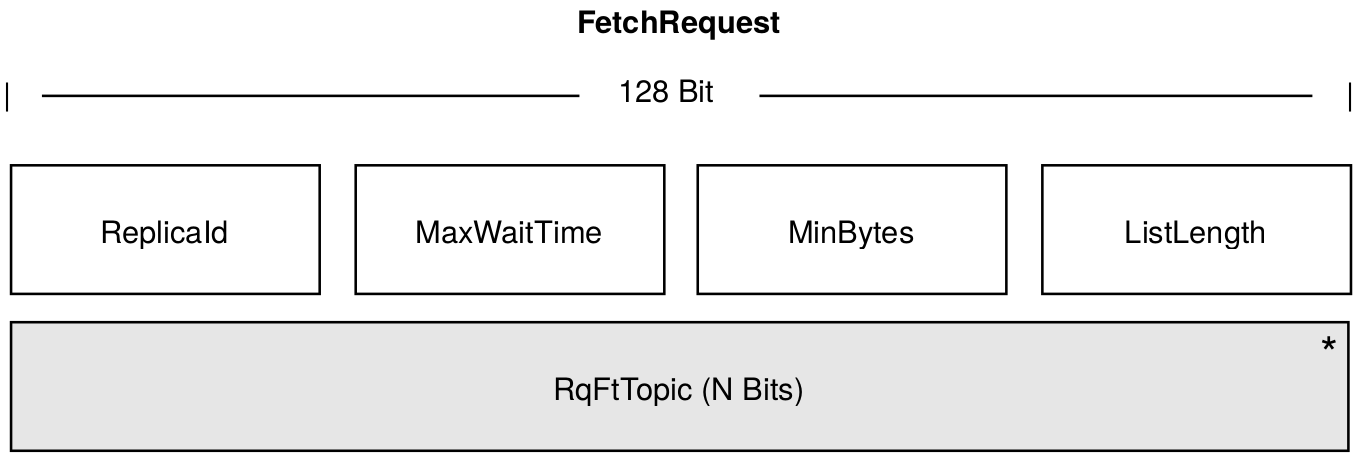
\includegraphics[width=0.7\textwidth]{images/impl-prot-types-fetchRequest.png}
    \caption{Format of type FetchRequest; * = N repetitions }
    \label{fig:impl-prot-types-fetchRequest}
\end{figure}

\begin{table}[H]
\centering
\begin{tabular}{ l  l  p{11cm} }
\hline
ReplicaId      & Data.Word32 & Indicates the node id of the replica initiating this request. (Not yet used in broker implementation)                        \\ \hline
MaxWaitTime    & Data.Word32 & Maximum amount of time in milliseconds to block,waiting if insufficient data is available at the time the request is,issued. \\ \hline
MinBytes       & Data.Word32 & Minimum number of bytes of messages that must be available to give a response.                                               \\ \hline
ListLength     & Data.Word32 & Number of elements in following list.                                                                                        \\ \hline
{[}FtTopics{]} & Data.List   & Sequence of FtTopics, see below                                                                                              \\ \hline
\end{tabular}
\end{table}

\begin{figure}[H]
    \centering
    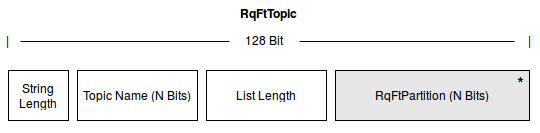
\includegraphics[width=0.7\textwidth]{images/impl-prot-types-ftTopic.png}
    \caption{Format of type RqFtTopic; * = N repetitions }
    \label{fig:impl-prot-types-ftTopic}
\end{figure}

\begin{table}[H]
\centering
\begin{tabular}{ l  l  p{10cm} }
\hline
StringLength      & Data.Word16     & Length, in bytes, of string TopicName.              \\ \hline
TopicName         & Data.ByteString & Name of the topic the fetch is for . \\ \hline
ListLength        & Data.Word32     & Number of element in following list.                \\ \hline
[FtPartition]     & Data.List       & Sequence of FtPartitions, see below.                \\ \hline
\end{tabular}
\end{table}

\begin{figure}[H]
    \centering
    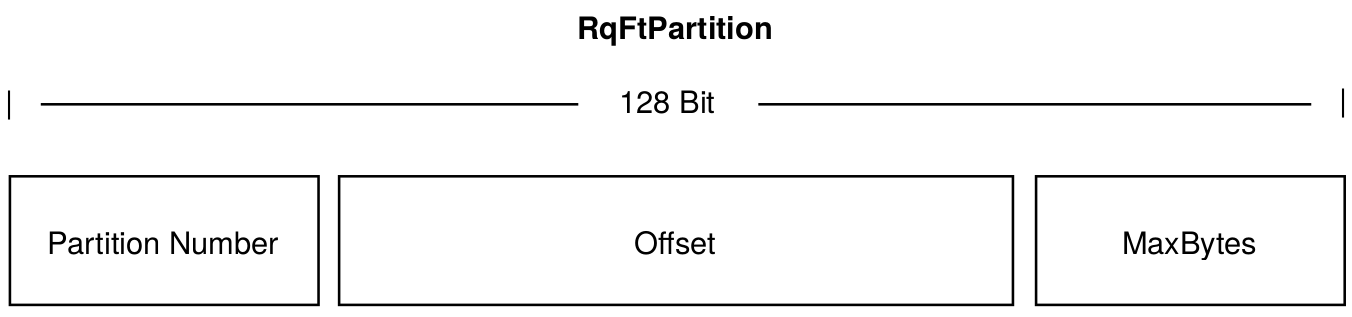
\includegraphics[width=0.7\textwidth]{images/impl-prot-types-ftPartition.png}
    \caption{Format of type RqFtPartition }
    \label{fig:impl-prot-types-ftPartition}
\end{figure}

\begin{table}[H]
\centering
\begin{tabular}{ l  l  p{10cm} }
\hline
PartitionNumber & Data.Word32 & Id of the partition the fetch is for.                                          \\ \hline
Offset          & Data.Word64 & Offset to begin the fetch from.                                                \\ \hline
MaxBytes        & Data.Word32 & Minimum number of bytes of messages that must be available to give a response. \\ \hline
\end{tabular}
\end{table}

\subsubsection{Metadata Request}
The request format for the metadata is fairly simple. Actually the
RequestMessage header with the appropriate APIkey suffices to initiate the
broker to reponse meta information about existing topics, partitions and
brokers. The request contains an optional list of topics, for which explicit
information is requested.

\begin{figure}[H]
    \centering
    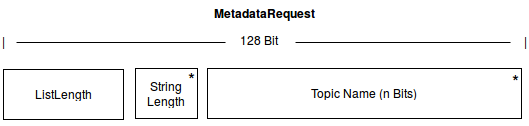
\includegraphics[width=0.7\textwidth]{images/impl-prot-types-metadataRequest.png}
    \caption{Format of type MetadataRequest, * = N repetitions}
    \label{fig:impl-prot-types-ftPartition}
\end{figure}

\begin{table}[H]
\centering
\begin{tabular}{ l  l  p{10cm} }
\hline
ListLength    & Data.Word32 & Number of element in following list.                                                                                             \\ \hline
StringLength      & Data.Word16     & Length, in bytes, of string TopicName.              \\ \hline
TopicName         & Data.ByteString & . The topic to produce metadata for. If
empty the request will yield metadata for all topics  \\ \hline
\end{tabular}
\end{table}

\subsection{Types related to Response}
A response message is the on-wire format of data which is getting from broker to
client.

Each request message has its same header fields independent for which API they are used. 
The real payload of the request is individual to the particular API which is
used. A response will always match the paired request (e.g. a ProduceResponse is
sent in return to a ProduceRequest).

\begin{figure}[H]
    \centering
    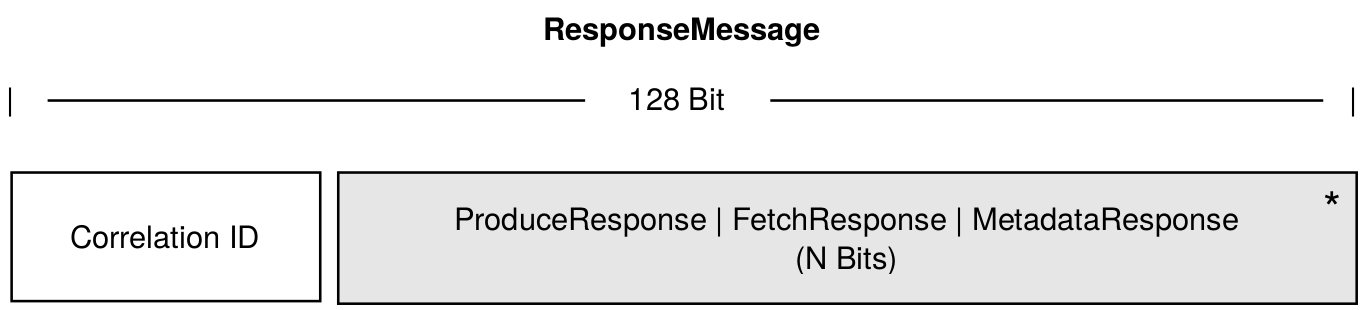
\includegraphics[width=0.7\textwidth]{images/impl-prot-types-responseMessage.png}
    \caption{Format of type ResponseMessage; * = N repetitions}
    \label{fig:impl-prot-types-responseMessage}
\end{figure}

\begin{table}[H]
\centering
\begin{tabular}{ l  l  p{10cm} }
\hline
CorrelationId  & Data.Word32 & Id that is supplied by request is passed back
(for request-reply reference).              \\ \hline
{[}Response{]} & Data.List   & Sequence of Responses of the same type (either
ProduceResponse, FetchResponse or others). \\ \hline
\end{tabular}
\end{table}


\subsubsection{ProduceResponse}
Response Payload for Produce API. Sends an ErrorCode which determines whether a
produce request for e specific topic-partition succeeded (ErrorCode 0 ) or ended
in a particular failure. 

\begin{figure}[H]
    \centering
    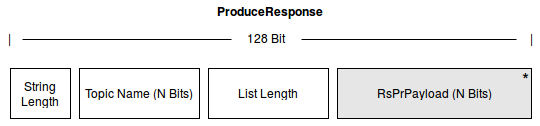
\includegraphics[width=0.7\textwidth]{images/impl-prot-types-produceResponse.png}
    \caption{Format of type ProduceResponse; * = N repetitions}
    \label{fig:impl-prot-types-produceResponse}
\end{figure}

\begin{table}[H]
\centering
\begin{tabular}{ l  l  p{10cm} }
\hline
StringLength      & Data.Word32     & Length, in bytes, of string TopicName. \\ \hline
TopicName         & Data.ByteString & Name of the topic this response entry corresponds to.\\ \hline
ListLength        & Data.Word32     & Number of element in following list.\\ \hline
{[}RsPrPayload{]} & Data.List       & Sequence of RsPrPayload, see below.
\\ \hline
\end{tabular}
\end{table}

\begin{figure}[H]
    \centering
    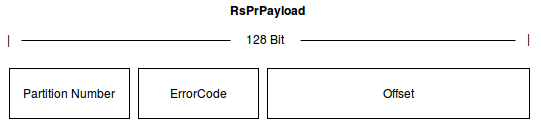
\includegraphics[width=0.7\textwidth]{images/impl-prot-types-prPayload.png}
    \caption{Format of type RsPrPayload, * = N repetitions}
    \label{fig:impl-prot-types-prPayload}
\end{figure}


\begin{table}[H]
\centering
\begin{tabular}{ l  l  p{10cm} }
\hline
PartitionNumber & Data.Word32 & Number of partition this response entry
corresponds to.                                                \\ \hline
ErrorCode       & Data.Word16 & Topic-Partition specific error code. Error code
0 determines that data has been published successfully. \\ \hline
Offset          & Data.Word64 & Number of element in following list.
\\ \hline
\end{tabular}
\end{table}

\subsubsection{FetchResponse}
Response Payload for Fetch API. Sends requested chunk of one ore more logs as
sequence of MessageSet's (see \ref{impl-protocol-types-data}). 

\begin{figure}[H]
    \centering
    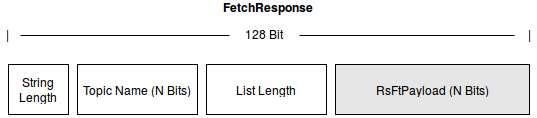
\includegraphics[width=0.7\textwidth]{images/impl-prot-types-fetchResponse.png}
    \caption{Format of type FetchResponse}
\end{figure}

\begin{table}[H]
\centering
\begin{tabular}{ l  l  p{10cm} }
\hline
StringLength      & Data.Word32     & Length, in bytes, of string TopicName. \\ \hline
TopicName         & Data.ByteString & Name of the topic this response entry corresponds to.\\ \hline
ListLength        & Data.Word32     & Number of element in following list.\\ \hline
{[}RsPrPayload{]} & Data.List       & Sequence of RsPrPayload, see below.
\\ \hline
\end{tabular}
\end{table}

\begin{figure}[H]
    \centering
    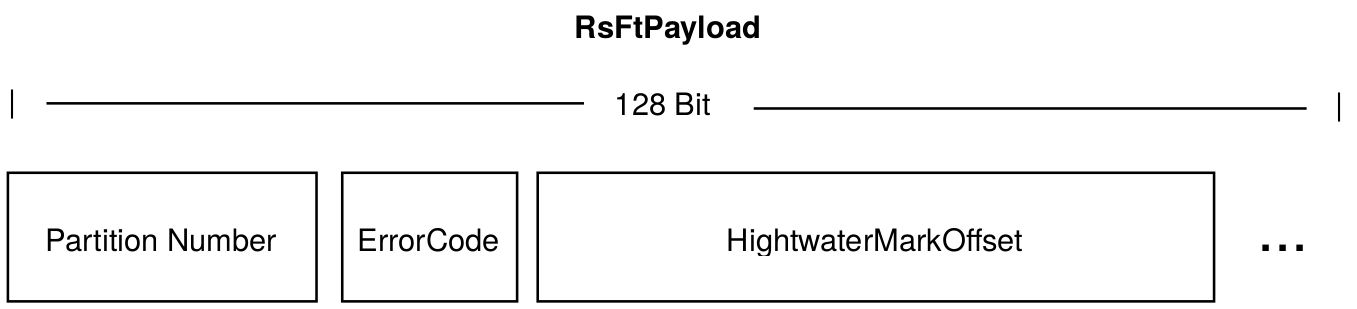
\includegraphics[width=0.7\textwidth]{images/impl-prot-types-ftPayload.png}
    \caption{Format of type RsFtPayload}
\end{figure}

\begin{table}[H]
\centering
\begin{tabular}{ l  l  p{10cm} }
\hline
PartitionNumber     & Data.Word32 & Number of partition this response entry corresponds to.                                                                                               \\ \hline
ErrorCode           & Data.Word16 & Topic-Partition specific error code. Error code 0 determines that data has been published successfully                                                \\ \hline
HighwaterMarkOffset & Data.Word64 & The offset at the end of the log for this partition. This can be used by,the client to determine how many messages behind the end of the log,they are \\ \hline
MessageSetSize      & Data.Word32 & The size in bytes of the message set for this topic-partition                                                                                         \\ \hline
{[}MessageSet{]}    & Data.List   & The message data fetched from this partition, in the format described below                                                                           \\ \hline
\end{tabular}
\end{table}

\subsubsection{Metadata Response}
As simple the metadata request is, the more complex the response format turns
out. It contains information about provided brokers, topics, partitions and
their replication status. 

\begin{figure}[H]
    \centering
    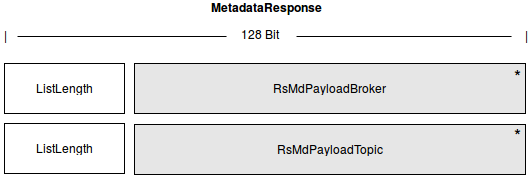
\includegraphics[width=0.7\textwidth]{images/impl-prot-types-metadataResponse.png}
    \caption{Format of type MetadataResponse, * = N repetitions}
\end{figure}

\begin{figure}[H]
    \centering
    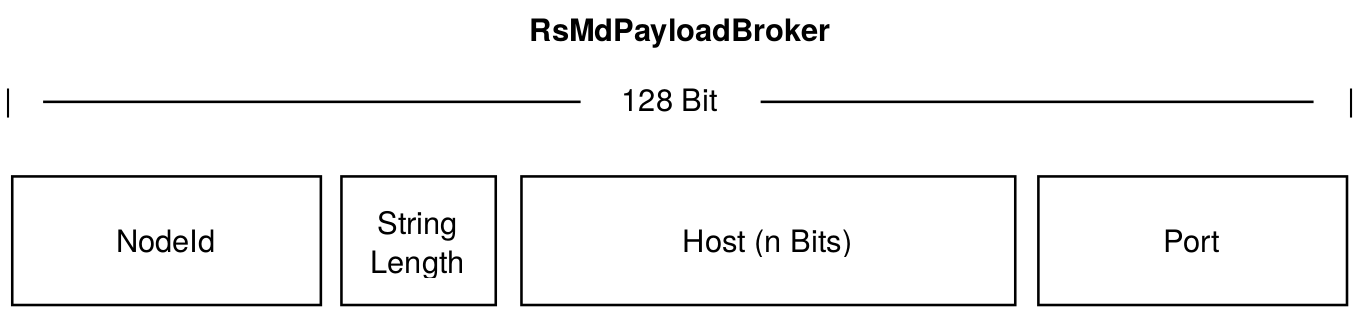
\includegraphics[width=0.7\textwidth]{images/impl-prot-types-mdPayloadBroker.png}
    \caption{Format of type RsMdPayloadBroker} 
\end{figure}

\begin{figure}[H]
    \centering
    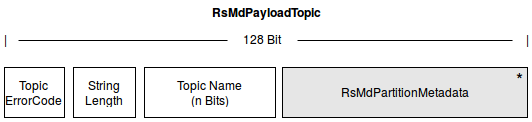
\includegraphics[width=0.7\textwidth]{images/impl-prot-types-mdPayloadTopic.png}
    \caption{Format of type RsMdPayloadTopic, * N repetitions} 
\end{figure}


\begin{table}[H]
\centering
\begin{tabular}{ l  l  p{10cm} }
\hline
ListLength        & Data.Word32     & Number of element in following list.\\ \hline
[RsMdPayloadBroker] & Data.List     & Sequence of RsMdPayloadBroker, contains
node Id, hostname and port information of broker.  \\ \hline
ListLength        & Data.Word32     & Number of element in following list.\\ \hline
[RsMdPayloadTopic] & Data.List     & Sequence of RsMdPayloadTopic, contains all,
or the requested topic names with approriate error code which determines status.
Also contains a sequence of RsMdPayloadMetadata, see below. \\ \hline
\end{tabular}
\end{table}

\begin{figure}[H]
    \centering
    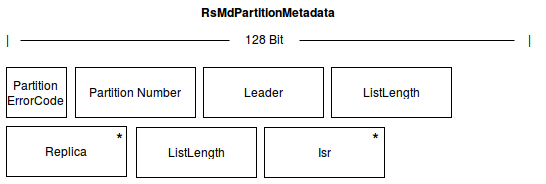
\includegraphics[width=0.7\textwidth]{images/impl-prot-types-mdPartitionMetadata.png}
    \caption{Format of type RsMdPartitionMetadata} 
\end{figure}

\begin{table}[H]
\centering
\begin{tabular}{ l  l  p{10cm} }
\hline
PartitionErrorCode  & Data.Word16 & Partition specific error code.                                                          \\ \hline
PartitionNumber     & Data.Word32 & Number of Partition this metadata is for.                                               \\ \hline
Leader              & Data.Word32 & The node id for the broker currently acting as leader for this partition.
                       If no leader exists because when beeinh in the middle of
                       a leader election this id will be -1.                                                                \\ \hline
ListLength        & Data.Word32     & Number of element in following list.                                                  \\ \hline
[Replicas]         & Data.List & The set of alive nodes that currently acts as
                       slaves for the leader for this partition, given as
                       Data.Word32.                                                                                        \\ \hline
ListLength        & Data.Word32     & Number of element in following list.                                                  \\ \hline
[Isr]   & Data.List   & The set subset of the replicas that are "caught up" to
                       the leader, given as Data.Word32.        \\ \hline
\end{tabular}
\end{table}


\subsection{Types related to Data}
\label{impl-protocol-types-data}
The actual transported data has a common structure,
called a MessageSet. This format happens to be used both for the on-disk storage on the
broker and the on-the-wire format. Therefore the broker do not need to perform
any transformations to the actual message when persisting to the log or read
from it. 

\begin{figure}[H]
    \centering
    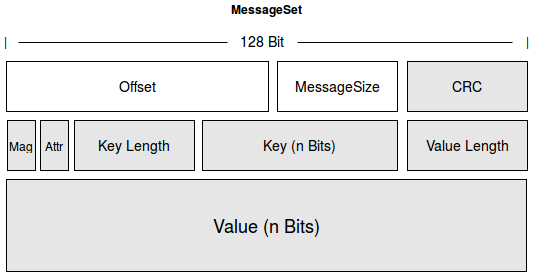
\includegraphics[width=0.7\textwidth]{images/impl-prot-types-messageSet.png}
    \caption{Format of type MessageSet including type Message and Payload}
    \label{fig:impl-prot-types-messageSet}
\end{figure}

\begin{table}[H]
\centering
\begin{tabular}{ l  l  p{11cm} }
\hline
Offset      & Data.Word64 & Determines log offset number in log.  When the producer is sending messages it doesn't actually know the offset and can fill in any value here it likes. \\ \hline
MessageSize & Data.Word32 & Determines size of Message in Bytes.               \\ \hline
Message     &     & Message format, see below.                                                                                                                    \\ \hline
\end{tabular}
\end{table}

\subsubsection{Message}
Message is part of the MessageSet and contains a checksum to check integrity of
the actual payload of the message. To abstract the fields which are checked we
combine them in another type, see Payload.

%\begin{figure}[H]
%    \centering
%    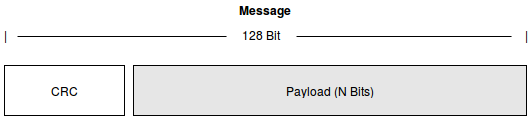
\includegraphics[width=0.7\textwidth]{images/impl-prot-types-message.png}
%    \caption{Format of type Message}
%    \label{fig:impl-prot-types-message}
%\end{figure}

\begin{table}[H]
\centering
\begin{tabular}{ l  l  p{11cm} }
\hline
CRC     & Data.Word32 & The CRC is the CRC32 of the remainder of the message bytes. This is used,to check the integrity of the message on the broker and consumer. \\ \hline
Payload &      & Payload format, see below.                                                                                                                  \\ \hline
\end{tabular}
\end{table}

\subsubsection{Payload}
This types defines the actual payload of a message with its meta info.

%\begin{figure}[H]
%    \centering
%    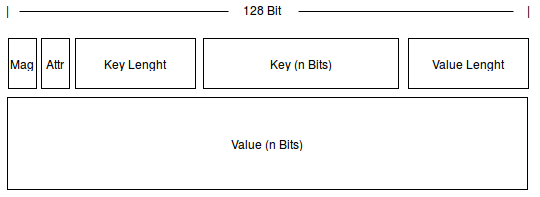
\includegraphics[width=0.7\textwidth]{images/impl-prot-types-payload.png}
%    \caption{Format of type Payload}
%    \label{fig:impl-prot-types-payload}
%\end{figure}

\begin{table}[H]
\centering
\begin{tabular}{ l  l  p{10cm} }
\hline
Magic       & Data.Word8      & This is a version id used to allow backwards compatible evolution of the message binary format. The current value is 0.                                         \\ \hline
Attributes  & Data.Word8      & This byte holds metadata attributes about the message. The lowest 2 bits,contain the compression codec used for the message. The other bits,should be set to 0. \\ \hline
KeyLen      & Data.Word32     & Determines length of Key field in bytes.                                                                                                                         \\ \hline
Key         & Data.ByteString & The key is an optional message key that is used for partition assignment. The key can be null.                                                                  \\ \hline
ValueLength & Data.Word32     & Determines length of Value field in bytes.                                                                                                                      \\ \hline
Value       & Data.ByteString & The actual message contents as an byte array. The message can be null. Kafka also supports recursive messages in which case 
                                the value may itself contain a message set. This
                                functionality is not implemented yet.                                                                                                                            \\ \hline
\end{tabular}
\end{table}

\section{Encode / Decode}

There are libraries in Haskell to encode or decode data to or from binary
format given as ByteString. As for binary serialization, the
\fnurl{Data.Binary}{https://hackage.haskell.org/package/binary-0.4.1/docs/Data-Binary.html}
library is being used as it works with lazy bytestrings. As an alternative to
Data.Binary, the cereal library
(\fnurl{Data.Serialize}{https://hackage.haskell.org/package/cereal-0.4.1.1/docs/Data-Serialize.html})
also provides binary serialization capabilities -- especially for strict
bytestrings. Lazy bytestring represent a list of bytes this plays nicely along
with streaming and thus for the use case of a message broker. Additionally,
lazy bytestrings support appending in O(1) complexity which will be used
frequently in the serialization process. This makes further usage of the
ByteString slightly more efficient.

Parsing libraries such as
\fnurl{Attoparsec}{https://hackage.haskell.org/package/attoparsec} or
\fnurl{Parsec}{https://hackage.haskell.org/package/parsec} where considered but
proved to not be suitable for performance critical applications. In fact, there
is no need for parsing functionality -- such as syntactic analysis -- regarding
the tasks the broker has to be capable of. 

\subsection{Decode Request/Response}

As mentioned in previous section, every request or response has the same header
fields. Functions are provided to either parsing a request or response and
remind of the original definition of the Kafka protocol as grammar. To identify
the actual type of request, the protocol describes an API Key field which holds
a numeric code which explicitly defines the type of request. Depending on the
API key, further parse functions will be called. 

The Get Monad (Data.Binary.Get) allows to comfortably parse ByteString in
it's big endian network order and decode it to appropriate types.

The following code shows the function for parsing an arbitrary request:

\begin{lstlisting}
import Data.Binary.Get

requestMessageParser :: Get RequestMessage 
requestMessageParser = do 
    apiKey        <- getWord16be
    apiVersion    <- getWord16be
    correlationId <- getWord32be
    clientIdLen   <- getWord16be
    clientId      <- getByteString $ fromIntegral clientIdLen
    request       <- case (fromIntegral apiKey) of
        0 -> produceRequestParser
        1 -> fetchRequestParser
        3 -> metadataRequestParser
        -- further API Codes 
        _ -> -- Invalid API Key 
    return $ RequestMessage apiKey apiVersion correlationId clientIdLen
    clientId request
\end{lstlisting}

Batched sequences are decodes as Data.List whereas the following function
provides a generic way to decode a list with given size and a parse each
element:
\begin{lstlisting}
parseList :: Int -> (Get a) -> Get [a]
parseList i p = do 
  if (i < 1) 
    then return []
    else do x <- p
            xs <- parseList (i-1) p
            return (x:xs)
\end{lstlisting}

%Because the format of a MessageSet is common for the transmission on wire as
%well for the persistence in the log we can use the same functions for both use cases:
%\begin{lstlisting}
%payloadParser :: Get Payload
%payloadParser = do
%  magic  <- getWord8
%  attr   <- getWord8
%  keylen <- getWord32be
%  paylen <- getWord32be
%  payload <- getByteString $ fromIntegral paylen
%  return $! Payload magic attr keylen paylen payload

%messageParser :: Get Message 
%messageParser = do 
%  crc    <- getWord32be
%  p      <- payloadParser
%  return $! Message crc p

%messageSetParser :: Get MessageSet 
%messageSetParser = do 
%  offset <- getWord64be
%  len <- getWord32be 
%  message <- messageParser
%  return $! MessageSet offset len message
%\end{lstlisting}

A batched sequence of MessageSets is a special case where the protocol does not provide a
field which determines the number of elements. There is just a field which contains
the size in bytes of all message sets. Therefore we implemented an according
list decoder for sequences of MessageSets:
\begin{lstlisting}
parseMessageSets :: Int -> Get [MessageSet]
parseMessageSets i = do
    if (i < 1)
    then return []
    else do x <- messageSetParser
            xs <- parseMessageSets $ i - (fromIntegral $ length $ buildMessageSet x)
            return $ (x:xs) 
\end{lstlisting}

Decoding a ByteString can be applied with \lstinline{runGet f b}, whereas
\lstinline{f} declares the parser function (indicated through Get a return type),
and  \lstinline{b} the bytestring to decode. This construct implies that the Get
monad is applied at latest possible point in time in constant complexity. For example: 
\begin{lstlisting}
import Data.Binary.Get

decodeRsMessage :: B.ByteString -> ResponseMessage
decodeRqMessage b = runGet requestMessageParser b

\end{lstlisting}


\subsection{Encode Request/Response}
\label{sec:impl-prot-encoding}
Obviously the encode module provides the opposite functionalities as the decode
module and was separated just for clarity. The implementation also rely on
\fnurl{Data.Binary}{https://hackage.haskell.org/package/binary-0.4.1/docs/Data-Binary.html}
and use the Put Monad (Data.Binary.Put) to construct ByteStrings.

The following code shows the function for encoding an arbitrary request:
\begin{lstlisting}
buildRqMessage :: RequestMessage -> Put
buildRqMessage e = do
  putWord32be $ rqSize e
  putWord16be $ rqApiKey e
  putWord16be $ rqApiVersion e
  putWord32be $ rqCorrelationId e
  putWord16be $ rqClientIdLen e
  putByteString $ rqClientId e
  case (fromIntegral $ rqApiKey e) of
    0 -> buildProduceRequest  $ rqRequest e
    1 -> buildFetchRequest    $ rqRequest e
    3 -> buildMetadataRequest $ rqRequest e
    -- further API Codes 
    _ -> -- Invalid API Key 
\end{lstlisting}

Batched sequences are encoded as Data.List whereas the following function
provides a generic way to build the list in given size and encode each element:
\begin{lstlisting}
buildList :: (a -> Put) -> [a] -> Put
buildList builder [] = putLazyByteString BL.empty
buildList builder [x] = builder x
buildList builder (x:xs) = do 
  builder x
  buildList builder xs
\end{lstlisting}

Encoding a ByteString can be applied with \lstinline{runPut f t}, whereas
\lstinline{f} declares the build function (indicated through Put return type),
and  \lstinline{t} the type to decode. Like with decoding, this construct
implies that the Put monad is applied at latest possible point in time in
constant complexity. For example: 
\begin{lstlisting}
import Data.Binary.Put

enodePrRqMessage :: RequestMessage -> B.ByteString
enodePrRqMessage r = runPut buildPrRqMessage r
\end{lstlisting}

\section{Client Library}
\label{sec:impl-prot-client}
As part of the protocol implementation, the client library provides an
API for clients to interact with the protocol. The goal is to isolate the
producer or consumer clients from implementations details of the types and
encode/decode functions. 

\subsection{Types}
The types provided by the client library give a simplified abstraction for
the types of the protocol implementation. All values which need to be
provided from a client are covered. Every type which is irrelevant to the client
is hide.

Depending on the API a client wants to access, either a Produce, Fetch of
Metadata type needs to be defined. Each of them consists of a Head, which
contains the header information every request needs to include. Furthermore, the
libary types allow the client to define nested sequences of topics and
partitions to fully support the batching approach of the Kafka protocol. 
\begin{lstlisting}
data Req = Produce Head [ToTopic] | Fetch Head [FromTopic] | Metadata Head [OfTopic]
data Head = Head
  { apiV      :: Int
  , corr      :: Int
  , client    :: BS.ByteString
  }
\end{lstlisting}

The following example shows the definition of a produce call to publish batched messages
for multiple topics and partitions. 

\begin{lstlisting}
  let head = Head 0 0 clientId
  let ms = [randBytes | x <- [1..10]]
  let req = Produce 
        head 
        [ToTopic topicA [ToPart 0 ms, ToPart 1 ms], ToTopic topicB [ToPart 0 ms]]
\end{lstlisting}

\subsection{Send Request}
Before sending an API call to the broker, the defined types above need to be
packed to the actual types of the Kafka protocol implementation (with all the
additional information which are hided from client). Therefore the client
library exposes a \lstinline{sendRequest} function. It packes the provided
\lstinline{Req} to the protocol conform \lstinline{RequestMessage} and encode it
to ByteString. Finally, the binary data is sent to the given socket.

\begin{lstlisting}
sendRequest :: Socket -> RequestMessage -> IO ()
sendRequest socket requestMessage = do
    SBL.sendAll socket msg
    where msg = runPut $ buildRqMessage $ pack requestMessage

class Packable a where
  pack :: a -> RequestMessage

instance Packable Req where
  pack (Produce head ts)  = packPrRqMessage head ts
  pack (Fetch head ts)    = packFtRqMessage head ts
  pack (Metadata head ts) = packMdRqMessage head ts

\end{lstlisting}

\subsection{Decode Response}
For parsing received responsed sent from broker, the client library exposes
functions for decoding the binary data. 

\begin{lstlisting}
To expose functionality for the client to decode responses sent from broker, the
client library provides specific decode functions: 

decodePrResponse :: BL.ByteString -> ResponseMessage
decodePrResponse a = runGet produceResponseMessageParser a

decodeFtResponse :: BL.ByteString -> ResponseMessage
decodeFtResponse b = runGet fetchResponseMessageParser b

decodeMdResponse :: BL.ByteString -> ResponseMessage
decodeMdResponse b = runGet metadataResponseMessageParser b
\end{lstlisting}

Instead of exposing the decode functions for response, it is conceivable to
provide unpack functionality which decodes the request and extracts relevant
fields to a simplified type structure (analog to sendRequest function above).

\newpage
\section{Testing}
For Haskell there are multiple frameworks for automated testing provided. To
test the functionality of the protocol implementation, \fnurl{hspec}
{https://hackage.haskell.org/package/hspec} is used. It provides good
integration within a cabal project (after setup run tests by simply call \lstinline{cabal test})
and generates useful tests logs to \lstinline{/dist/test/}. It also supports
interoperability to other frameworks like
\fnurl{HUnit}{https://hackage.haskell.org/package/HUnit}.

Major approach in the implemented tests is to determine if the encode and decode
functions are corresponding. Therefore a given type (e.g. ProduceRequest) is
encoded to bytestring and afterwards decoded back to the type. Is the resulting
type equals to the original, than the process was successful. This helps to
determine wrong or missing instruction in encoding/decoding when protocol
changed. The goal is also to easily test abnormal input or varying
for example the size of lists from zero to N elements. To simplify code of
single tests, type fixtures are implemented. The fixtures helps to assemble
types together from different fixtures whereas their fields are already filled
with some sample values. 

The following code shows an extract of the protocol tests:
\begin{lstlisting}
import Test.Hspec
import SpecFixtures

spec :: Spec
spec = do
  describe "Kafka.Protocol" $ do
    context "MessageSet" $ do
      it "Test1: Default Value" $ do
        let ms = getMessageSetFixture $ getMessageFixture $ getPayloadFixture "Test"
        testMs ms
      it "Test2: No Value" $ do
        let ms = getMessageSetFixture $ getMessageFixture $ getPayloadFixture ""
        testMs ms
      it "Test3: JSON like Value" $ do
        let ms = getMessageSetFixture $ getMessageFixture $ getPayloadFixture
           "[ obj : { value : 123 }]"
        testMs ms

testMs :: MessageSet -> Expectation
testMs m = (runGet messageSetParser $ runPut $ buildMessageSet m) `shouldBe` m

\end{lstlisting}




